\documentclass{../source/zjureport}

\major{信息工程}
\name{周灿松}
\title{实验设计报告}
\stuid{3190105055}
\college{信息与电子工程学院}
\date{\today}
\lab{东4-223}
\course{数字系统设计实验}
\instructor{屈民军、唐奕}
\grades{}
\expname{实验设计报告}
\exptype{设计实验}
\partner{}

\begin{document}
    \makecover
    \makeheader

    \section{实验目的和要求}
        \subsection{实验目的}
        \begin{enumerate}
            \item 掌握音符产生的方法,了解DDS技术的应用
            \item 了解音频编解码的应用
            \item 掌握系统"自顶向下"的数字系统设计方法
        \end{enumerate}

        \subsection{实验要求}
        设计出一个能够播放四首乐曲的音乐播放器,满足如下两个要求:
        \begin{enumerate}
            \item 设置play/pause_button、next_button、reset三个按键.play/pause_button按键实现乐曲在暂停与播放之间切换,按下next_button可以播放下一首乐曲;
            \item 设置3个LED灯,LED0显示目前的播放状态(亮为播放,灭为暂停),LED1和LED2显示目前乐曲号
        \end{enumerate}

    \section{实验内容和原理}
        \subsection{主控制器模块}
            \subsubsection{设计说明}
            主控制器模块主要作用为响应用户按键信息、控制系统播放两大任务,算法流程图和书上类似,此处不表。
            \subsubsection{主控制器代码}
            \lstinputlisting[
                language = Verilog,
                caption = 主控制器模块代码
                 ]{code/mcu.v}
        
        \subsection{song_reader模块}
            \subsubsection{设计说明}
            song_reader模块任务如下:
            \begin{enumerate}
                \item 根据mcu模块的要求,选择播放乐曲。
                \item 响应note_player模块请求,从song_rom中逐个取出音符{note, duration}送给note_player模块播放
                \item 判断乐曲是否播放完毕,若播放完毕,则回复mcu模块应答信号。
            \end{enumerate}


            我们采用了书上给出的电路结构实现了上述功能,其中song_rom模块是一个只读存储器,用于存放乐曲;地址计数器计算播放的音符数,它的进位输出作为;结束判断模块利用地址计数器进位输出和从song_rom中取出的duration判断是否输出song_done信号。

            \subsubsection{结束判断模块设计}
            结束判断模块采用了老师建议的状态机方法实现:


            一、地址计数器进位输出co作为reset信号,duration单独输入,共四个状态实现,代码如下:
\begin{lstlisting}[
    caption=判断结束模块一,
    language = Verilog
    ]
//判断乐曲是否播放结束模块
module is_over (
    input [5:0] duration ,
    input reset , clk ,
    output reg done
);
    parameter RESET = 0 , PAUSE = 1 , PLAY = 2 , OUT = 3;
    reg [1:0] state=0 , nextstate;

    always @(posedge clk) begin
        if(reset) state = RESET;
        else state = nextstate;
    end

    always @(*) begin
        done = 0;
        case (state)
            RESET:begin
                done = 1;
                nextstate = PAUSE;
            end 
            PAUSE:begin
                done = 0;
                if(duration)begin
                    nextstate = PLAY;
                end
                else nextstate = PAUSE;
            end
            PLAY:begin
                done = 0;
                if(duration) nextstate = PLAY;
                else nextstate = OUT;
            end
            OUT:begin
                done = 1;
                nextstate = PAUSE;
            end
        endcase
    end
endmodule
\end{lstlisting}


            二、听了老师的讲解之后,意识到将两个信号按"duration == 0 || co"进行输入状态机会更加简单,如是将代码简化至如下:
\begin{lstlisting}[
    caption=判断结束模块二,
    language = Verilog
    ]
//判断乐曲是否播放结束模块
module is_over (
    input [5:0] duration ,
    input reset , clk ,
    output reg done
);
    parameter RESET = 0 , PAUSE = 1 , PLAY = 2 , OUT = 3;
    reg [1:0] state=0 , nextstate;

    always @(posedge clk) begin
        if(reset) state = RESET;
        else state = nextstate;
    end

    always @(*) begin
        done = 0;
        case (state)
            RESET:begin
                done = 1;
                nextstate = PAUSE;
            end 
            PAUSE:begin
                done = 0;
                if(duration)begin
                    nextstate = PLAY;
                end
                else nextstate = PAUSE;
            end
            PLAY:begin
                done = 0;
                if(duration) nextstate = PLAY;
                else nextstate = OUT;
            end
            OUT:begin
                done = 1;
                nextstate = PAUSE;
            end
        endcase
    end
endmodule
\end{lstlisting}

            \subsubsection{song_reader模块代码}
\begin{lstlisting}[
    caption=song_reader模块,
    language = Verilog
    ]
    module song_reader (
        input clk,reset,play,note_done,
        input [1:0] song,
        output reg new_note,
        output song_done,
        output [5:0] note , duration
    );
        //状态编码
        parameter RESET = 0 , NEW_NOTE = 1 , WAIT = 2 , NEXT_NOTE = 3;
        reg [1:0] state , nextstate;
    
        wire [4:0] lowaddr;//song_rom的低五位地址
        wire judge;//歌曲结束标志一
        
        //控制器时序部分
        always @(posedge clk) begin
            if(reset) state = RESET;
            else state = nextstate;
        end
    
        //控制器组合部分
        always @(*) begin
            //默认输出
            new_note = 0;
            case (state)
                RESET:begin
                    new_note = 0;
                    if(play) nextstate = NEW_NOTE;
                    else nextstate = RESET;
                end
                NEW_NOTE:begin
                    new_note = 1;
                    nextstate = WAIT;
                end  
                WAIT:begin
                    new_note = 0;
                    if(play == 0) nextstate = RESET;
                    else if(note_done) nextstate = NEXT_NOTE;
                    else nextstate = WAIT;
                end
                NEXT_NOTE:begin
                    new_note = 0;
                    nextstate = NEW_NOTE;
                end
            endcase
        end
    
        //实例化地址计数器
        counter_n #(.n(32) , .counter_bits(5)) addrCounter(.clk(clk) , .r(reset) , .en(note_done) , .q(lowaddr) , .co(judge));
        
        //实例化song_rom,取出音符
        song_rom song_rom(.clk(clk) , .dout({note,duration}) , .addr({song,lowaddr}));
    
        //实例化判断模块
        over is_over(.signal((duration==0)||co) , .reset(reset) , .clk(clk) , .done(song_done));
    
    endmodule
\end{lstlisting}

    \subsection{note_player模块}
        \subsubsection{设计说明}
        音符播放模块note_ player是本实验的核心模块,它主要任务包括以下几方面。
        \begin{enumerate}
            \item 从 song_reader模块接收需播放的音符{note, duration}
            \item 根据note值找出DDS的相位增量k
            \item 以48kHz速率从 Sine_rom取出正弦样品送给音频编解码器接口模块
            \item 当一个音符播放完成,向song_reader模块索取新的音符
        \end{enumerate}
        进一步划分模块可将note_player划分为一下各个模块:作为控制单元的控制器、记录音符标记note和DD模块相位增量k查找表关系的FreqROM、DDS模块、音符节拍计时器。

        下面给出DDS模块、节拍计时器、note_player代码

        \subsubsection{代码}
        \lstinputlisting[
            language = Verilog,
            caption = DDS模块
        ]{code/dds.v}

        \lstinputlisting[
            language = Verilog,
            caption = 节拍计时器
        ]{code/timer.v}

        \begin{lstlisting}[
            caption=note_player模块,
            language = Verilog
            ]
module note_player (
    input clk , reset , play_enable , 
    input [5:0] note_to_load,duration_to_load,
    input load_new_note,sampling_pulse,beat,
    output reg note_done,
    output [15:0] sample,
    output sample_ready);
    //状态编码
    parameter RESET = 0 , WAIT = 1 , DONE = 2 , LOAD = 3;
    reg [1:0] state , nextstate;
            
    reg timer_clear , load;
    wire timer_done;
    wire [5:0] addr;
    wire [19:0] klow;
            
    always @(posedge clk) begin
        if(reset) state = RESET;
        else state = nextstate;
    end
            
    always @(*) begin
        //默认状态
        timer_clear = 1 ; load = 0 ; note_done = 0;
                    
        case (state)
            RESET:begin
                timer_clear = 1 ; load = 0 ; note_done = 0;
                nextstate = WAIT;
            end  
            WAIT:begin
                timer_clear = 0 ; load = 0 ; note_done = 0;
                if(play_enable == 0) nextstate = RESET;
                else if(timer_done) nextstate = DONE;
                else if(load_new_note) nextstate = LOAD;
                else nextstate = WAIT;
            end
            DONE:begin
                timer_clear = 1 ; load = 0 ; note_done = 1;
                nextstate = WAIT;
            end
            LOAD:begin
                timer_clear = 1 ; load = 1 ; note_done = 0;
                nextstate = WAIT;
            end
        endcase
    end
            
    //实例化音符节拍定时器
    timer #(.counter_bits(6)) timer1(.clk(clk) , .en(beat) , .r(timer_clear) , .done(timer_done) , .n(duration_to_load));          
            
    //实例一个D寄存器
    dffre #(.n(6)) D(.d(note_to_load) , .en(load) , .r(~play_enable||reset) , .clk(clk) , .q(addr));
            
    //实例化FreqROM
    frequency_rom FreqROM(.clk(clk) , .dout(klow) , .addr(addr));
            
    //实例化DDS
    dds DDS(.K({2'b00,klow}) , .clk(clk) , .reset(~play_enable||reset) , .sampling_pulse(sampling_pulse) , .sample(sample) , .new_sample_ready(sample_ready));
                
endmodule
        \end{lstlisting}

    \subsection{同步化电路}
        \subsubsection{设计说明}
        因为音频解码接口模块和其他模块采用了不同的时钟,我们需要将二者进行同步化
        \subsubsection{代码}
        \lstinputlisting[
            language = Verilog,
            caption = 同步化电路
        ]{code/synch.v}

\section{主要仪器设备}
\begin{enumerate}
    \item 装有 Vivado和 ModelSim SE软件的计算机。
    \item Nexys Video Artix-7 FPGA多媒体音视频智能互联开发系统。
    \item 有源音箱或耳机。
\end{enumerate}

\section{操作方法和实验步骤}
\begin{enumerate}
    \item 按照书中提供的框图,将音乐播放器次顶层划分为一下几个模块:主控制器、乐曲读取、音符播放、同步化电路以及节拍基准产生器
    \item 参考实验15的资料,学习DDS技术相关知识,编写DDS模块并进行仿真
    \item 根据书上的指导,依次编写剩下模块并进行仿真验证,测试其是否符合要求
    \item 编写次顶层模块,并在其中设置参数sim方便仿真
    \item 新建Vivado工程,生成符合要求的DCM模块,将自己编写的模块以及老师提供的网表文件及接口文件加入工程。对工程进行综合、约束、实现,并下载到开发板中进行验证
\end{enumerate}

\section{实验数据记录和处理}
    \subsection{DDS模块}
        \subsubsection{仿真图}
        \begin{figure}[htp]
            \centering
            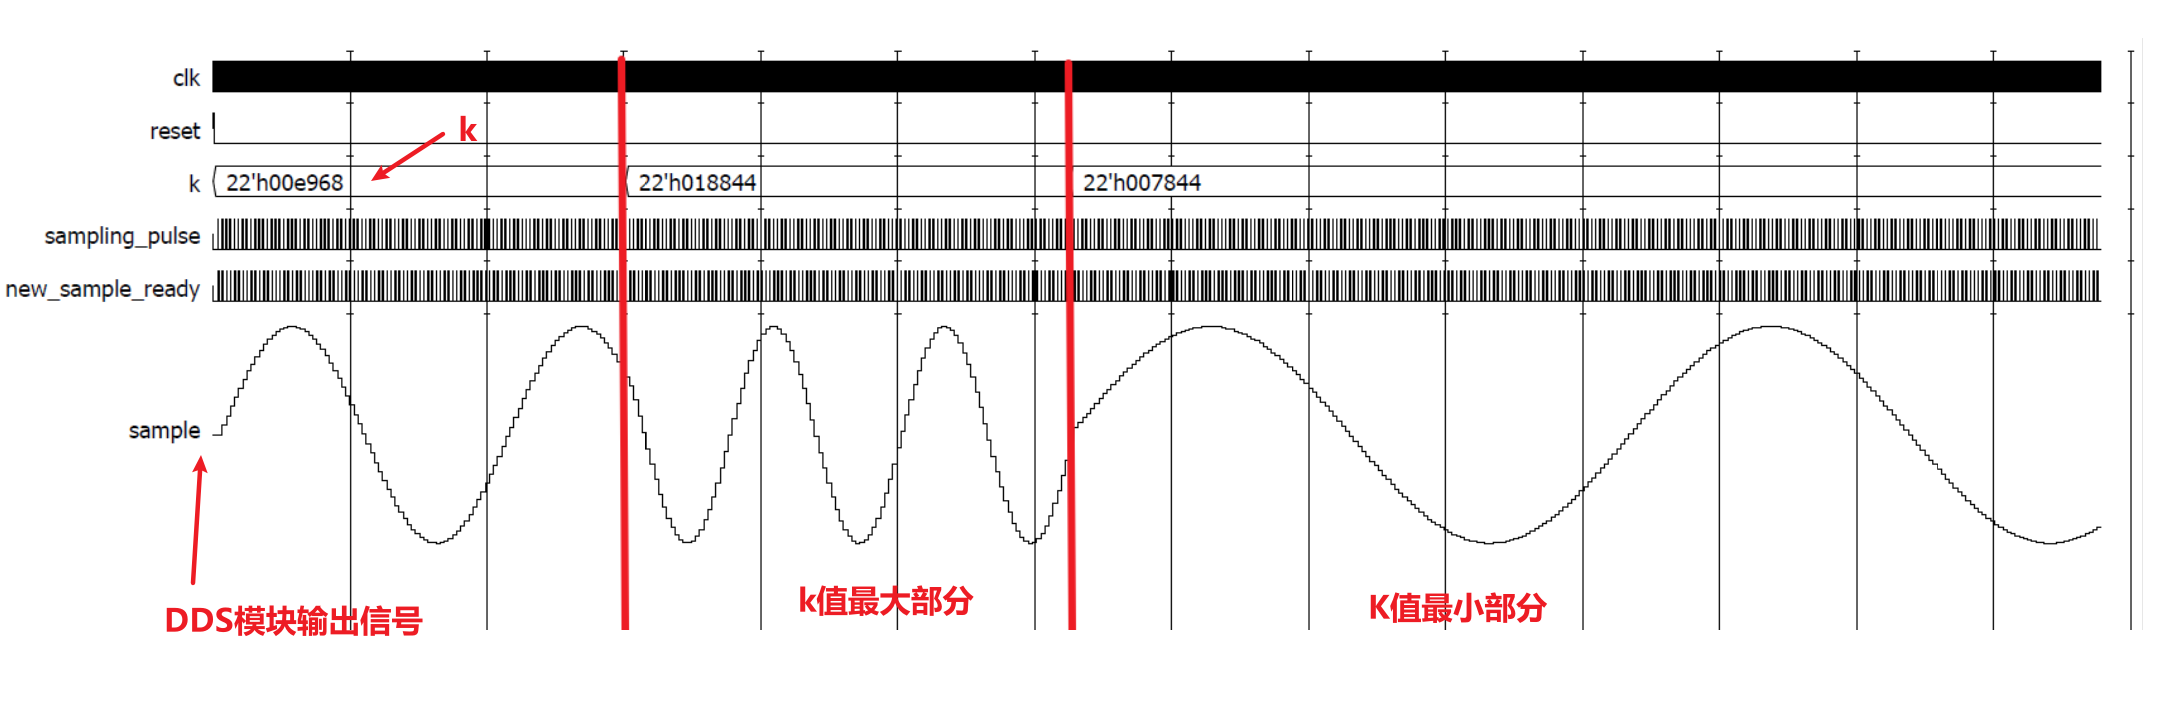
\includegraphics[width = 0.9\textwidth]{dds.png}
            \caption{DDS模块仿真图}
        \end{figure}

        \subsubsection{结果分析}
        由图可见,随着k值增大,sample信号频率逐渐增大,符合DDS模块要求

    \subsection{mcu模块}
        \subsubsection{仿真图}
        \begin{figure}[htp]
            \centering
            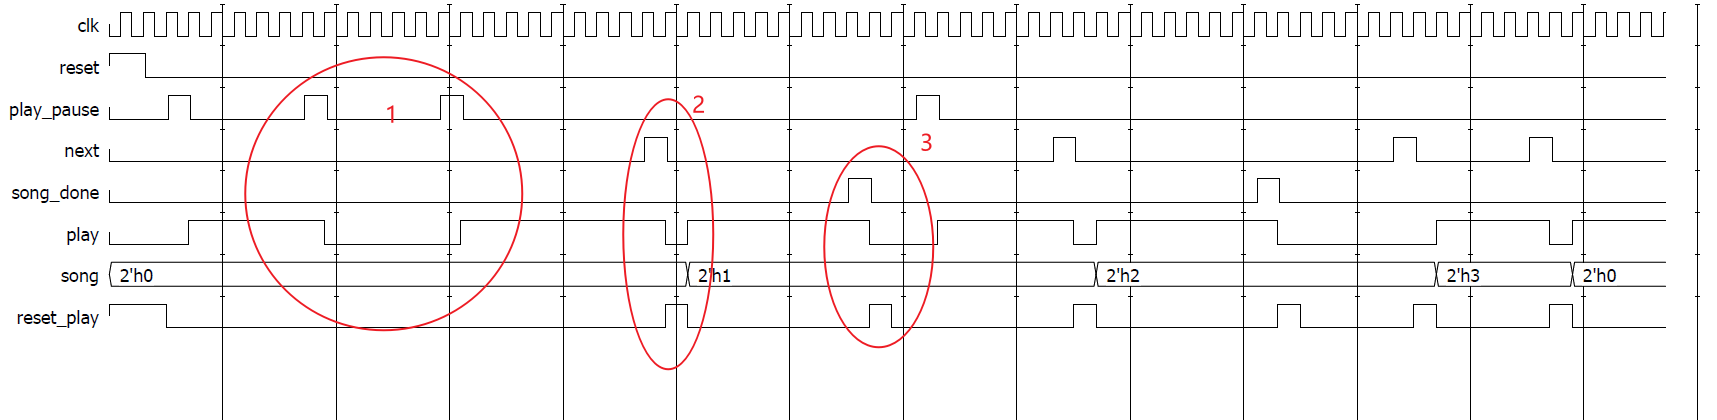
\includegraphics[width = 0.9\textwidth]{mcu.png}
            \caption{MCU模块仿真图}
        \end{figure}

        \subsubsection{结果分析}
        由圆圈1中波形可知,play_pause信号工作正常,能够正常输出play信号;由源泉2中波形可知,next信号工作正常;由圆圈3中波形可知,歌曲结束时的切换正常
        \newpage

    \subsection{song_reader模块}
        \subsubsection{仿真图}
        \begin{figure}[htp]
            \centering
            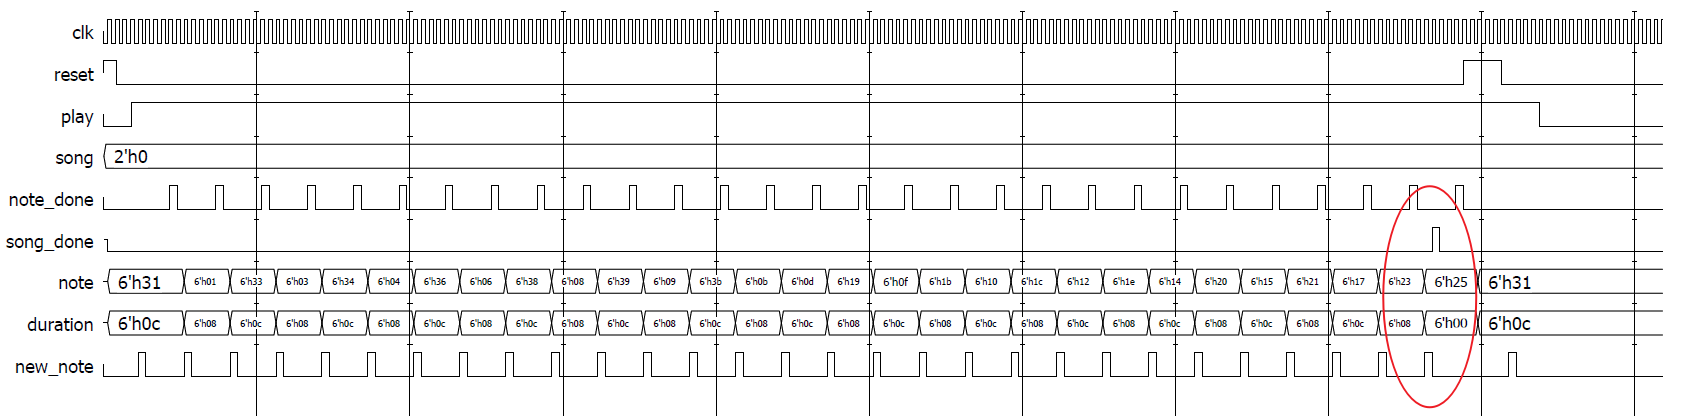
\includegraphics[width = 0.9\textwidth]{songreader.png}
            \caption{song_reader模块仿真图}
        \end{figure}

        \subsubsection{结果分析}
        由波形图中可以看出,当输入音符的duration为0时,song_reader模块能够正确输出一个song_done信号,符合设计要求
    
    \subsection{note_player模块}
        \subsubsection{仿真图}
        \begin{figure}[htp]
            \centering
            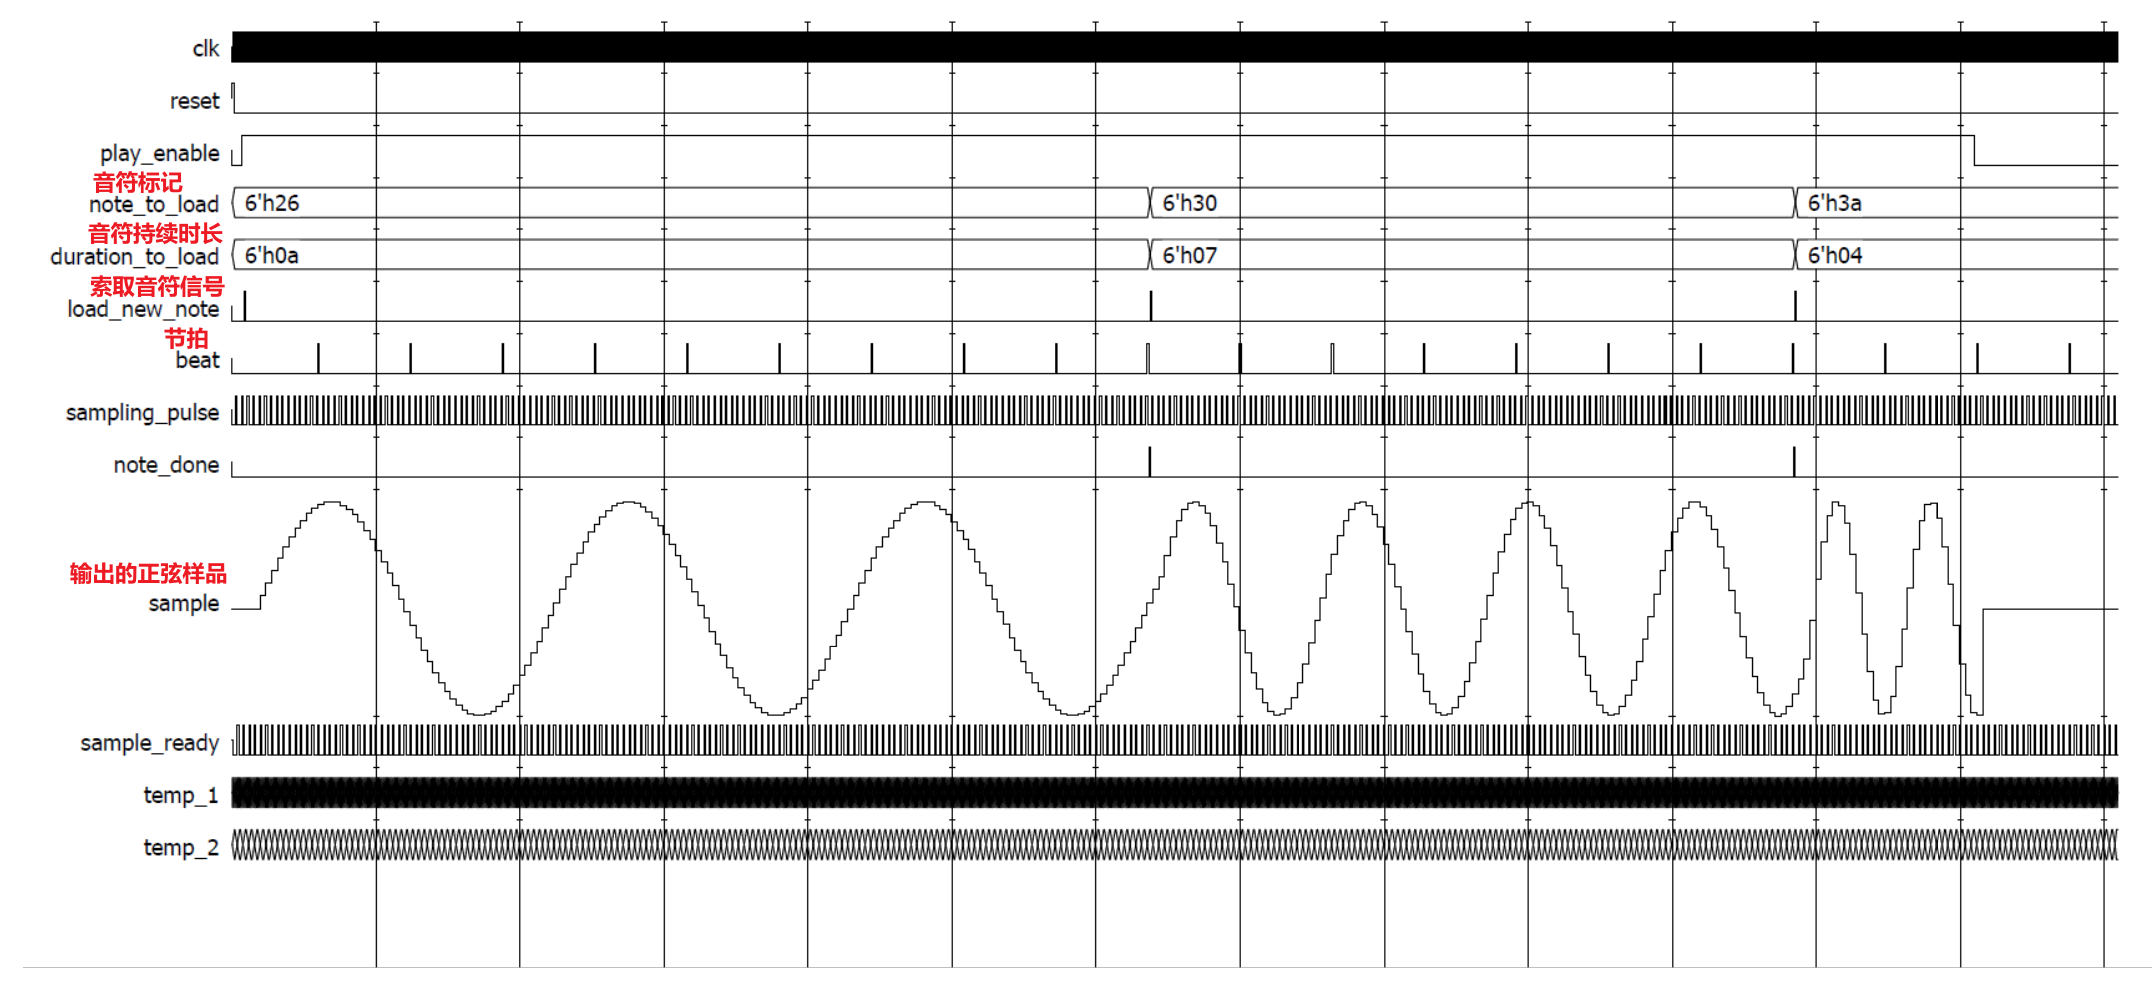
\includegraphics[width = 0.9\textwidth]{noteplayer.png}
            \caption{note_player模块仿真图}
        \end{figure}

        \subsubsection{结果分析}
        由上图可以发现,sample信号的频率随着note_to_load信号的增大而逐渐增大,同时观察信号改变时经历的beat信号数目,可以发现是和duration_to_load相等的,同时在一个音符结束之后也会输出一个note_done,说明note_player模块正常。

    \subsection{次顶层}
        \subsubsection{仿真图}
        \begin{figure}[htp]
            \centering
            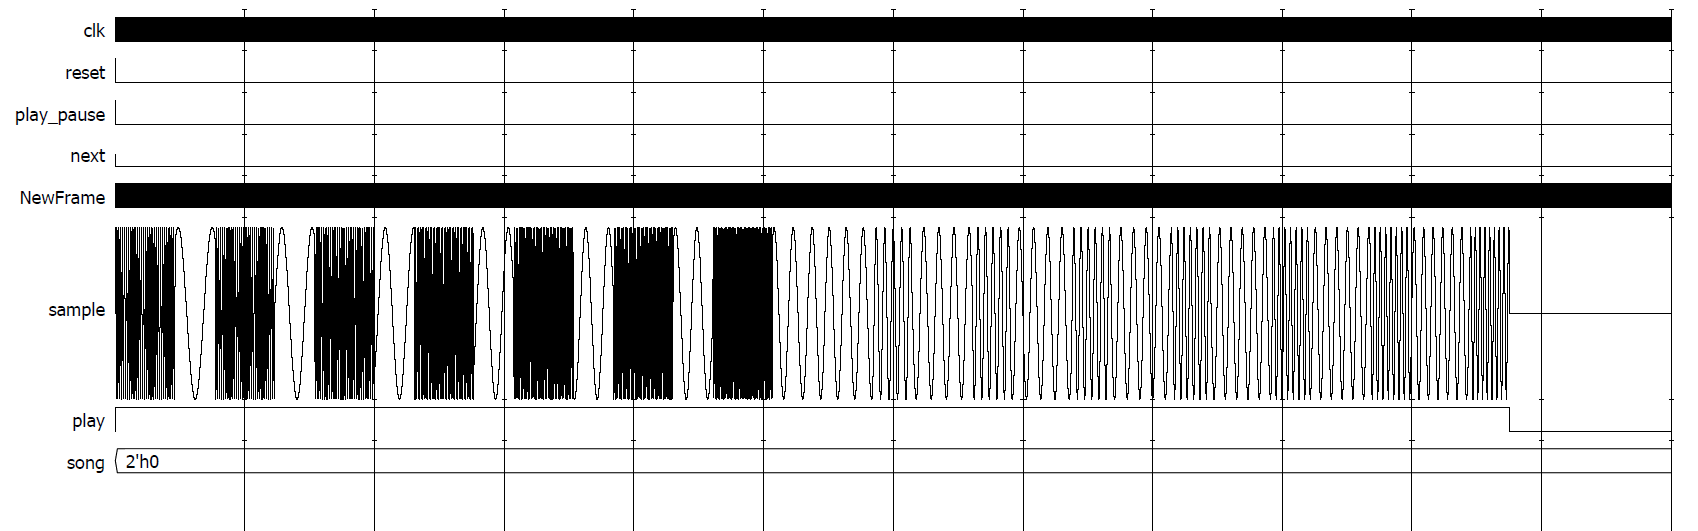
\includegraphics[width = 0.9\textwidth]{top.png}
            \caption{次顶层模块仿真图}
        \end{figure}

        \subsubsection{结果分析}
        和书上仿真结果对比,可以看出符和要求,次顶层工作正常
    
    \subsection{Vivado上板测试}
    通过仿真图可以看出,各个模块工作均正常,达到了预期的工作效果,组合而成的次顶层模块仿真结果也与预期相同。


    在vivado中生成二进制流上板测试后,经过调试song_reader模块中的结束判断模块,最终实现了所有的预期功能。

\section{思考题}
    \subsection{在实验中,为什么 next_button 、 play_pause_button 两个按键需要消颤动及同步化处理,而reset 按键不需要消颤动及同步化处理?}
    reset信号为复位信号,当reset=1后,系统内部已经完成复位。后续reset信号无论为0或者1,对系统而言并没有影响,所以可以不对reset信号进行消颤动及同步化处理。

    但是next_button 、 play_pause_button信号的值不同会影响系统状态的转换。如果next_button不进行消颤动及同步化处理,系统可能会接收到很多个next_button信号,这就会导致跳过了很多首歌,无法达到切换下一首的目标;同理,如果play_pause_button不进行相应处理,会导致歌曲断断续续,不够连贯。不仅达不到预期效果,同时更会加剧系统的损耗

    \subsection{在主控制器(mcu)设计中,是否存在接收不到按键信息?若存在,概率多大?有没必要修改设计?}
    存在。在RESET->PAUSE以及NEXT->PLAY状态切换的过程中,mcu无法接收到按键输入。因为这两个状态都只有一个始终节拍,所以概率很好,没有必要修改设计。

\section{心得体会}
本次实验带给我的第一个感受就是完事开头难。相比于前面做的实验,这个实验无论是代码量还是难度都是远超其余实验的,而且数电实验书也不像前面几个实验的部分一样保姆级教程,使得我最开始拿到题目的时候不知道从何处开始。最终,花费了一个下午加一个晚上搞懂了DDS模块的原理以及完成了响应代码的编写,在DDS模块过了测试之后,顿时就对这个实验有了更多的信心。于是,在接下来的一天里,通过学习教材并不断试错,最终用半天时间完成了第一版代码的编写。


在编写各个模块的过程中,逐步体会到了什么叫做“自顶向下”的系统设计方法。采用这种方法设计系统时,能够很明白地理清各个模块之间的关系,而且由于各个模块都是相对独立的,在调试的时候也会更加简单,可以通过分析实验中反映出的各种信息初步得知是哪一个模块出了问题,改bug的时候也更加简单。同时,由于模块相对独立,也更加不容易出现牵一发而动全身的连锁反应。

当然,在本次实验中也遇到了以下两个主要问题:
\begin{enumerate}
    \item 春学期做实验的时候过于急功近利,导致没有打好基础。在拿到音乐播放器项目时一时陷入了茫然,不知从何处下手,最终通过从头学习前几次实验的代码,一步步地理解各个操作的含义,解决了这一问题。这一问题也让我意识到在学习一个新的知识时,不管它看上去有多简单,也不能够急功近利地不去理解,基础没打好后续一定会让你付出更加惨重的代价。
    \item song_done模块由于结束判断没有做好始终不对。最开始我并没有认真阅读老师的课件,凭借着自己的“勇气”一头扎进了代码编写之中,忽视了结束判断的重要性,在上板调试的时候浪费了接近一个上午解决这一问题,最终还是屈老师指出了我的这一问题。在此感谢屈老师耐心解答我这一问题,后续认真学习了这个实验才知道这个问题是有多不应该。在懂了结束判断模块的编写方法后,我采用了将地址计数器和duration信号分别输入同一状态机进行处理的方案,最终虽然能够正常运行,但是状态机也显得过于复杂,不那么容易让人理解,后面旁听屈老师给别的同学讲解这一模块的编写时的思路让我明白了如何设计更加简洁的状态机,这也是为什么在我的song_reader模块里面会有over与is_over两个模块的原因。
\end{enumerate}

除了以上两个主要问题,当然也有变量名写错、数据传输错误之类的小错误,在这一类错误里,最值得人注意的就是变量名写错,因为modelsim仿真时这类错误不会报错,所以在实例化各个模块时一定要仔细。

至于在这次实验中的收获,我觉得除了对Verilog语言的熟悉,更重要的是这次试验让我学会了踏踏实实地做事,不要妄想一步登天,还有就是学会了如何管理自己的文件。

\end{document}